\documentclass[12pt,fleqn]{article}
\usepackage[portuguese]{babel}
\usepackage{xiiiemc}
\usepackage{natbib}
\usepackage{fancyhdr}
\usepackage{color}
\usepackage{wallpaper} 
\usepackage{titlesec}   %% Define space between paragraph e section
\usepackage{float} 	%% Use to fix Figure or Table: ex: \begin{table}[H]
\usepackage{listings}
\usepackage{listingsutf8}
\usepackage{graphics}
\usepackage{subfigure}
\usepackage{siunitx}
\usepackage{verbatim}
\usepackage{caption}
\usepackage{tikz}
\usepackage{pgfplots}
\pgfplotsset{width = 7cm,compat=1.14}
\usepackage[hyphens]{url}
\usepackage[all]{xy}
\urlstyle{same}
\lstset{
  literate=% %configuration alfabeth  brazilian 
  {\'a}{{\'a}}1
  {\'i}{{\'i}}1
  {\~a}{{\~a}}1
  {\^a}{{\^a}}1
  {\^e}{{\^e}}1,
  basicstyle = \small,
  mathescape % math mode
}

%%%%Don't edit this block. It reduces the spacing between the lines of the references
\let\OLDthebibliography\thebibliography
\renewcommand\thebibliography[1]{\OLDthebibliography{#1} \setlength{\parskip}{0pt}\setlength{\itemsep}{0pt plus 0.3ex}}
%%-----------------------------------------------EDIT-----------------------------------------------
  \title{ESTUDO COMPUTACIONAL SOBRE OS PONTOS CR\'ITICOS DE DEMANDA ENERG\'ETICA PARA  MODELO HIDROT\'ERMICO}%%-----------------------------------------------EDIT----------------------------------------------
\author
    {\rm \begin{tabular}{l} 
    \textbf{Jefferson Bezerra dos Santos}$^{1}$ - {\textnormal jeffersonsantos@ppgmmc.ci.ufpb.br}\\%
    \textbf{A definir}$^{2}$ - {\textnormal e-mail}\\
    \textbf{A definir}$^{3}$ - {\textnormal e-mail}\\
    {\fontsize{11}{0}\selectfont $^{1}$Universidade Federal da Para\'iba, Centro de Inform\'atica, Jo\~ao Pessoa,
  PB, Brasil}\vspace*{-0.05cm} \\
    {\fontsize{11}{0}\selectfont $^{2}$}\vspace*{-0.05cm}\\
    {\fontsize{11}{0}\selectfont $^{3}$}
  \end{tabular}}
%%----------------------------------------------------------------------------------------------

\fancypagestyle{firspagetstyle}
{
	\lhead{}
	\fancyhead[C]{%
		\includegraphics[width=1\linewidth]{logo}\\%
		{\scriptsize \fontfamily{phv}\fontseries{b}\selectfont \color[rgb]{0.45,0.45,0.45}
		08 a 11 de Outubro de 2019\\
		Universidade Federal de Juiz de Fora\\
		Juiz de Fora - MG\\
	    }
	}
	\renewcommand{\headrulewidth}{0.0pt}
	\fancyfoot[C]{\footnotesize \parbox{15cm} {\centering  \fontsize{7.5}{0}\selectfont \it Anais do XXII ENMC – Encontro Nacional de Modelagem Computacional e X ECTM – Encontro de Ciências e Tecnologia de Materiais\\Juiz de Fora, MG – 08 a 11 Outubro 2019}} % \ttfamil
	\rhead{}
}

\begin{document}
\maketitle
\thispagestyle{firspagetstyle}

\fancyhead[L]{\footnotesize{\fontsize{7.5}{0}\selectfont \it XXII ENMC e X ECTM\\
	08 a 11 de Outubro de 2019\\
	Universidade Federal de Juiz de Fora – Juiz de Fora - MG\\}}
\renewcommand{\headrulewidth}{0.0pt}
\fancyfoot[C]{\footnotesize \parbox{15cm} {\centering  \fontsize{7.5}{0}\selectfont \it  Anais do XXII ENMC – Encontro Nacional de Modelagem Computacional e X ECTM – Encontro de Ciências e Tecnologia de Materiais\\Juiz de Fora, MG – 08 a 11 Outubro 2019}} % \ttfamil
\rhead{}

\begin{abstract}
  Com o aumento da demanda por energia el\'etrica e o apelo das fontes renov\'aveis, grandes avan\c cos tecnol\'ogicos
  s\~ao indispens\'aveis para um crescimento eficiente e sustent\'avel. No Brasil a hidrel\'etrica \'e a principal fonte de gera\c c\~ao de energia. No entanto, devido ao aumento desproporcional da demanda e a escassez de chuvas, tem sido necess\'ario a ativa\c c\~ao de termel\'etricas para suprir a demanda. Consequentemente, isto acarreta em um aumento na fatura
  dos consumidores resid\^enciais. Neste contexto, este trabalho tem como finalidade analisar, as consequ\^encias que o aumento da demanda
  associado a problemas energ\'eticos, podem ocasionar no gerenciamento do balan\c co energ\'etico. Vislumbrando a necessidade de realizar um gerenciamento adequado do despacho de energia, de modo a minimizar os custos da gera\c
  c\~ao e uma diminui\c c\~ao do impacto ambiental, neste trabalho foi proposto um estudo baseado em Programa\c c\~ao
  Din\^amica Dual Estoc\'astica para sistemas hidrot\'ermicos (hidrel\'etricas e termel\'etricas).
\end{abstract}

\palavra {\em{Energia, Efici\^encia energ\'etica, Demanda, Sustentabiliade, Planejamento.}}
\pagestyle{fancy}

\section{INTRODU\c C\~AO}
A crecente necessidade pelo atendimento \`a demanda tem ocasionado um aumento da complexidade dos
sistemas de gera\c c\~ao de energia el\'etrica. Em contrapartida, a pesquisa por uma gera\c c\~ao de energia que favore\c
ca o desenvolvimento sustent\'avel tornou-se um dos principais temas debatidos no cen\'ario internacional. O sistema brasileiro \'e constitu\'ido predominante por um sistema interligado
hidrot\'ermico, tendo como caracter\'iticas principais o interc\^ambio de energia entre regi\~oes e a possibilidade de
complementaridade existente entre as hidr\'eletricas e as term\'eletricas Tolmasquim (2016). Em um planejamento hidrot\'ermico os aspectos
de relev\^ancia s\~ao: acoplamento espacial, acoplamento temporal e a estocasticidade dos reservat\'orios. Em cada
est\'agio do planejamento \'e necess\'aria a tomada de decis\~ao fazendo-se a escolha pela quantidade gerada de energia
proveniente das term\'eletricas e das hidr\'eletricas. Neste
contexto, atualmente destaca-se a Programa\c c\~ao Din\^amica Dual
Estoc\'atica (PDDE), pois possibilita uma flexibilidade para a descri\c c\~ao do acoplamento temporal e espacial existente entre as
usinas hidrel\'etricas, al\'em de permitir o  planejamento em v\'arios cen\'arios de aflu\^encias proporcionando-se a
modelagem da incerteza dos reservat\'orios. Contudo, dependendo do n\'umero elevado e das quantidades de cen\'arios  para o planejamento
nem sempre \'e poss\'ivel que a t\'ecnica de PDDE obtenha uma configura\c c\~ao \'otima para todos os cen\'arios
considerados tornando-se sua principal desvantagem.

Diversos trabalhos na literatura utilizam a PDDE como forma de planejamento. Um estudo recente da t\'ecnica
de constru\c c\~ao de \'arvore cen\'arios para a PDDE pode ser encontrado em (Rebennack
,2016). O estudo sobre modelamento hidrot\'ermico n\~ao convexo utilizando PDDE para n\~ao linearidades envolvendo reservat\'orio de
hidr\'eletricas \'e encontrado em (Cerisola \& Latorre \& Ramos,
2011). E uma an\'alise comparativa entre Programa\c c\~ao Din\^amica Primal Estoc\'astica e PDDE para modelo
hidrot\'ermico de longo prazo \'e descrita em (Martinez \&
Soares, 2004). 

O presente estudo propõe a analisar os pontos cr\'iticos de demanda em modelos hidrot\'ermicos que utilizam a PDDE.
Tendo como intuito verificar quais as consequ\^encias que varia\c c\~oes na demanda podem ocasionar na configura\c c\~ao
desses sistemas, al\'em de elencar os poss\'iveis fatores que sofreram com as mudan\c cas ocorridas no intuito de obter
um planejamento energ\'etico eficiente. Este trabalho \'e
subvidido da seguinte maneira: Na Se\c c\~ao 2 foi abordada a configura\c c\~ao do despacho do Brasil; Na se\c c\~ao 3
\'e abordada a Programa\c c\~ao Din\^amica Dual Estoc\'astica; Na se\c c\~ao 4 \'e abordada a an\'alise das simula\c
c\~oes; Na se\c c\~ao 5 as conclu\~oes do presente estudo. 

\section{DESPACHO DE ENERGIA}
A an\'alise dos fatores que envolvem a matriz energ\'etica brasileira sobre os aspectos relacionados \`a demanda e a
oferta \'e bastante
complexa. Um dos principais elementos que ocasionam empecilho \'e a depend\^encia h\'idrica que ocorre no setor energ\'etico brasileiro (Tolmasquim, 2016). O equil\'ibrio entre oferta e demanda n\~ao \'e apenas conseguido com um aumento de oferta,
\'e necess\'aria uma atua\c c\~ao tamb\'em na demanda. Uma vez que a demanda possui uma forte rela\c c\~ao com o
desenvolvimento de um pa\'is envolvendo aspectos como o acesso que a popula\c c\~ao possui aos servi\c cos de
infra-estrutura,
recebendo destaque para o saneamento b\'asico, os transportes, as comunica\c c\~oes e a energia (Atlas de
energia el\'etrica no Brasil, 2008). 

De maneira geral, historicamente o setor energ\'etico convive com dois grandes extremos de uma lado a
pesquisa por efici\^encia energ\'etica e por outro lado proporcionar que a popula\c c\~ao tenha acesso  a essas inova\c
c\~oes tecnol\'ogicas. Diante desse desafio, o Brasil possui o Sistema Interligado Nacional (SIN) que corresponde as
regi\~oes Sul, Sudeste, Centro-Oeste, Nordeste e parte do Norte. Sendo o respons\'avel por abrigar cerca de $96,6\%$ de toda a capacidade de produ\c c\~ao de energia do Brasil (Atlas de
energia el\'etrica no Brasil, 2008). Uma das vantagens da ado\c c\~ao do SIN deve-se a possibilidade de interc\^amcio
energ\'etico, isto \'e, regi\~oes que sofrem com problemas no abastecimento  de energia devido algum motivo externo
podem ser auxiliadas por outras regi\~oes. Uma outra possibilidade \'e a opera\c c\~ao de usinas hidrel\'etricas e termel\'etricas no
regime de complementaridade, ou seja, as termel\'etricas s\~ao ativadas para a suprir demanda quando por algum motivo as
hidrel\'etricas n\~ao possuem condi\c c\~oes evitando-se preju\'izos na oferta. O sistema de energia brasileiro tamb\'em \'e constituido pelos sistemas isolados localizados principalmente na regi\~ao Norte,
estados como Amazonas, Roraima, Acre, Amap\'a e Rond\^onia. Sua denomina\c c\~ao deve-se por n\~ao estarem interligados ao
SIN e por n\~ao permitirem um interc\^ambio com outras regi\~oes devido as caracter\'isticas geogr\'aficas. O
funcionamento dos
sistemas isolados \'e predominantemente t\'ermico. Os custos para a gera\c c\~ao de energia nesses sistemas s\~ao
superiores ao SIN (Atlas de
energia el\'etrica no Brasil, 2008). Portanto, o sistema brasileiro \'e constitu\'ido pelo SIN e pelos sistemas isolados. 

 A produ\c c\~ao de eletricidade no sistema brasileiro tem como objetivo principal minizar
os custo de opera\c c\~ao e garantir o suprimento de energia em todo o pa\'is (Tolmasquim, 2016). Pelo SIN ser
constitu\'ido predominantemente por um sistema hidrot\'ermico este \'e afetado pela incerteza associada a pluviosidade
das regi\~oes que o constituem (Atlas de
energia el\'etrica no Brasil, 2008). No entanto, a demanda do sistema deve ser garantida de forma a n\~ao prejudicar o
abastecimento ao mesmo tempo o custo associado aos sistemas isolados necessita ser considerado para n\~ao ocasionar um
aumento desagr\'avel no pre\c co  associado ao sistema de energia de uma forma geral. 
Neste contexto, o planejamento eficiente do sistema energ\'etico observando caracter\'isticas como, demanda, oferta e
  as configura\c c\~oes do sistema \'e conhecido na literatura como o despacho de energia. Para sistemas
 hidrot\'ermicos as caracter\'isticas do despacho podem ser resumidas no dilema do
 ``operador'' dado pelo diagrama a seguir.
 \begin{figure}[!h]
  \xymatrix@=0.2em{
	& & *+[F]{\text{CHUVA}} \ar[r]& *+[F]{\text{DECIS\~AO CORRETA}}\\
	& *+[F]{\text {USAR \ RESERVAT\'ORIO}} \ar[ur] \ar[dr] & &\\
	& & *+[F]{\text{SECA}} \ar[r] & *+[F]{\text{PREJU\'IZO}} \\
	*+ [F]{\text {OPERADOR}} \ar[uur] \ar[ddr] & & & \\
	& & *+[F]{ \text {CHUVA}} \ar[r] & *+ [F]{\text{PREJU\'IZO}}\\
	& *+ [F]{\text {USAR TERMEL\'ETRICA}} \ar[ur] \ar[dr]& &\\
	& & *+[F] {\text {SECA}} \ar[r] & *+[F]{\text{DECIS\~AO CORRETA}}
 }
 \caption {Dilema do operador.}  
 \label{fig1}
 \end{figure}

Conforme o diagrama o operador do sistema pode ter preju\'izo associado a sua escolha dada a estocasticidade dos
reservat\'orios das hidrel\'etricas. Dada a complexidade do sistema hidrot\'ermico
brasileiro este tipo de decis\~ao possui um grau de dificuldade bastante elevado. Nesta perspectiva um dos modelos de
planejamento desenvolvido para lidar com a tomada de decis\~ao de curto prazo foi desenvolvido pelo o Centro de
Pesquisas de Energia El\'etrica (Cepel), o Modelo de Planejamento de Sistemas Interligados de
Curto Prazo (DECOMP). Esse modelo fundamenta-se na t\'ecnica conhecida na literatura como Programa\c c\~ao Din\^amica
Dual Estoc\'astica.

\section{Programa\c c\~ao Din\^amica Dual Estoc\'astica}
\subsection{Otimiza\c c\~ao}
No planejamento de um sistema energ\'etico hidrot\'ermico as caracter\'isticas b\'asicas s\~ao manter as metas de gera\c c\~ao para suprir a demanda e minizar o valor esperado do custo de
opera\c c\~ao ao longo do per\'iodo de estudo. As caracter\'isticas mencionadas configuram o despacho de energia
. Dadas as possibilidades de configura\c c\~oes poss\'iveis para o sistema deseja-se obter a combina\c
c\~ao na qual o valor do custo
associdado seja m\'inimo. Portanto, o despacho de energia trata-se de um problema de otimiza\c c\~ao. No estudo da
teoria da otimiza\c c\~ao existe uma fun\c c\~ao $f$ ao qual deseja-se obter
quando poss\'ivel seu minimizador a fun\c c\~ao $f$ poder\'a ter minimizador
global (G), sendo tamb\'em poss\'ivel a exist\^encia de minizador local (L) para a intersec\c c\~ao  de uma vizinhan\c ca U
de pontos de $f$ com conjunto $D$ de restri\c c\~oes do problema (Izmailov \& Solodov, 2014). Um entendimento intuitivo
pode ser dado pela figura a seguir.

\begin{figure}[!h]
  \centering
\begin{tikzpicture}
  \draw [->, thick, black] (0,0)--(8,0) node[right] {$x$};
  \draw [->, thick, black] (0,0)--(0,4) node[above] {$f$};
  \draw [thick, black] (0,1)--(1,3);
    \draw [thick, black] (1,3)--(2,0.5) node[above1,xshift = 3,yshift = 16] {$\text{G}$};
  \draw [thick, black](2,0.5)--(4,3);
  \draw [thick, black](4,3)--(5,2) node[below left] {$\text{L}$};
  \draw [thick, black](5,2)--(6,3)--(8,3)node[above,yshift=8] {$\text{D}$};
  \draw [ultra thick, black](2,0.5) circle (0.5mm);
  \draw [ultra thick, black](5,2) circle (0.5mm);
  \draw [ultra thick, black](5,2) circle (0.5mm);
  \draw [dashed, black](5,2) circle (1.0cm) node[above,yshift = 8] {$U$}; 
  \draw [dashed, black](2,0.5)--(0,0.5) node[left] {$f(x_g)$};
  \draw [dashed, black](2,0.5)--(2,0) node[below] {$x_g$};
  \draw [dashed, black] (1.5,1.8)--(1.5,0) node[below] {$x_1$};
  \draw [dashed, black] (1.5,1.8)--(0.0,1.8) node[left] {$f(x_1)$};
  \draw [dashed, black](3.8,2.7)--(3.8,0) node[below] {$x_2$};
  \draw [dashed, black](3.5,2.7)--(0.0,2.7) node[above left] {$f(x_2)$};
  \draw [dashed, black](5,2)--(0,2) node[above left] {$f(x_l)$};
  \draw [dashed, black](5,2)--(5,0) node[below] {$x_l$};
\end{tikzpicture}
\caption{Minimizador global(G) e local (L),conjunto (D) sem restri\c c\~oes} 
\label{fig2}
\end{figure}
Pela Figura (\ref{fig2}) nota-se a diferen\c ca existente entre minizador global e local para $f$. Para todo
ponto $x$ de $f$ que esteja no conjunto D \'e verdadeira a afirma\c c\~ao $f(x_g) \leq f(x)$, portanto $G$ configura-se o minizador global para
$f$, por outro lado a afirma\c c\~ao $f(x_l) \leq f(x)$ n\~ao \'e verdadeira para todo o $x$ escolhido, sendo verdadeira apenas
para um subconjunto de elementos na intersec\c c\~ao de uma vizinha\c ca $U$ de $x_l$ com o conjunto $D$ de restri\c
c\~oes. Neste caso,
$L$ \'e um minizador local para $f$. No exemplo em Figura (\ref
{fig2}) considerou-se todos os pontos de $f$ sem nenhuma restri\c c\~ao para o conjunto. Contudo, em certas ocasi\~oes
\'e necess\'ario que no processo de encontrar o minizador
esse deve satisfazer  determinadas restri\c c\~oes, por exemplo, $x > x_d$ esse tipo de caso pode ser observado na
figura a seguir.  

\begin{figure}[!h]
  \centering
\begin{tikzpicture}
  \draw [->, thick, black] (0,0)--(8,0) node[right] {$x$};
  \draw [->, thick, black] (0,0)--(0,4) node[above] {$f$};
  \draw [thick, black] (0,1)--(1,3);
  \draw [thick, black] (1,3)--(2,0.5) node[left] {$\textbf{G}$};
  \draw [thick, black](2,0.5)--(4,3);
  \draw [thick, black](4,3)--(5,2) node[below] {$ \textbf{L}$};
  \draw [thick, black](5,2)--(6,3)--(8,3);
  \draw [ultra thick, black](2,0.5) circle (0.5mm);
  \draw [ultra thick, black](4.5,0) circle (0.1mm) node[below]{$x_d$};
  \draw [ultra thick, black](5,2) circle (0.5mm);
  \fill [black, draw=black, opacity = 0.4] (4.5,0) rectangle (8,4) node[above] {$\textbf{D}$};
  \draw [thick, black](5,0) circle (0.2mm) node[below] {$x_l$};
  %\draw [dashed, black](5,2) circle (1.0cm) node[above,yshift = 8] {$U$}; 
  \draw [dashed, black](2,0.5)--(0,0.5) node[left] {$f(x_g)$};
  \draw [dashed, black](2,0.5)--(2,0) node[below] {$x_g$};
  \draw [dashed, black] (1.5,1.8)--(1.5,0) node[below] {$x_1$};
  \draw [dashed, black] (1.5,1.8)--(0.0,1.8) node[left] {$f(x_1)$};
  \draw [dashed, black](3.8,2.7)--(3.8,0) node[below] {$x_2$};
  \draw [dashed, black](3.5,2.7)--(0.0,2.7) node[above left] {$f(x_2)$};
  \draw [dashed, black](5,2)--(0,2) node[above left] {$f(x_l)$};
  \end{tikzpicture}
  \caption{M\'inimo global (G), e minizador global (L),(D) com restri\c c\~oes.} 
\label{fig3}
\end{figure}
O minizador conforme figura \ref{fig3} deve satisfazer a restri\c c\~ao $x > x_d$. Apesar do ponto
$G$ ser o m\'inimo de $f$, contudo por n\~ao pertence ao conjunto D de restri\c c\~oes n\~ao ser\'a o minizador. Neste
caso o ponto L \'e o minizador global, pois $f(x_l) \leq f(x)$ para todo $x$ de $f$ que esteja no conjunto
$D$. O conjunto no qual s\~ao definidas as restri\c c\~oes para o problema de otimiza\c c\~ao receber o nome
de conjunto vi\'avel j\'a o minimizador do problema de
otimiza\c c\~ao dado o conjunto vi\'avel $D$ esse \'e conhecido como ponto de \'otimo sua nomenclatura
comum \'e dada por ${x}^{*}$. Dadas as ideias intuitivas os
conceitos formais podem ser abordados de forma a evitar qualquer tipo de ambiguidade. Desta
forma, dados os conjuntos $D \subset {R}^{n}$ e $\Psi \subset {R}^{n}$ tal que $D
\subset \Psi $ e existe uma fun\c c\~ao $f: \Psi \subset R$. O objetivo \'e encontrar o minizador para
$f$ no conjunto  vi\'avel $D$ a fun\c c\~ao $f$ recebe o nome de fun\c c\~ao objetivo (Izmailov \& Solodov, 2014). De forma equivalente pode-se
representar o problema por,
\begin{equation}
  \text{min} \ f(x) \ \text{sujeito a $x \in D$},
  \label {min1}
\end{equation}
onde dado o ponto $\overline{x} \in D$ este \'e,
\begin{itemize}
  \item minimizador global, se \\
	$f(\overline{x}) \leq f(x) $ qualquer que seja $x \in D$, 
  \item minimizador local, se \\ 
	$f(\overline{x}) \leq f(x)$ qualquer que seja $x \in D \cap U$,
	onde $U$ \'e uma vizinhan\c ca de $x$.
\end{itemize}
sendo ${x}^{*}$  o minizador procurado pertencendo ao conjunto de restri\c
c\~oes D. Para o presente estudo \'e suficiente considerar o conjunto $D$ como sendo um conjunto poliedral. De uma forma bem grosseira a ideia seria evitar
poss\'iveis ``fissuras'' em nosso conjunto de restri\c c\~oes. Um conjunto  \'e dito poliedral quando \'e poss\'ivel sua representa\c c\~ao como um conjunto das solu\c c\~oes de um
sistema finito de equa\c c\~oes e inequa\c c\~oes lineares (Izmailov \& Solodov, 2014), por exemplo,
\begin{equation*}
  D = \left\{ x \in {R}^{n}; Ax = a, Bx \leq b\right\},
\end{equation*}
onde $A \in R(l,m)$, $B \in R(m,n)$, $a \in {R}^{n}$, e $b \in {R}^{m}$ adotando-se que $R(l,m)$ representar o
espa\c co de matrizes com $l$ linhas, e $m$ colunas. Dada que $f$ em Eq.(\ref {min1}) \'e uma fun\c c\~ao linear e $D$ um conjunto
poliedral na teoria da otimiza\c c\~ao problemas deste tipo s\~ao problemas de Programa\c c\~ao Linear, por exemplo, o despacho de energia
para o caso determin\'istico pertence a essa categoria. Por fim, para problemas de otimiza\c c\~ao de uma forma geral o conceito de dualidade \'e
essencial. Considerando-se um problema de Programa\c c\~ao Linear que ser\'a chamado de problema primal,
\begin{equation}
  \text{min} \left < c,x \right > \ \text{sujeito a} \ x \in D = \left\{ x \in {R}^{n}; Bx \geq b \right\}, 
  \label{min2}
\end{equation}
onde $B \in R(m,n), c \in {R}^{n}$ e $b \in {R}^{n}$ onde ``$< >$'', representar o produto interno Euclidiano.
O problema dual para Eq. (\ref{min2}) \'e definido por,
\begin{equation}
  \text{max} \left < b, \mu \right > \ \text{sujeito a} \ \mu \in \Delta = \left\{ \mu \in R_+^m;
  {B}^{T} \mu = c \right\}.
\end{equation}

A grande import\^ancia da dualidade para a Programa\c c\~ao Linear deve-se ao fato que em certas circunst\^ancias o valor \'otimo do problema dual \'e equivalente ao do
problema primal e na maioria do casos o problema dual possui uma estrutura menos complexa (Izmailov \& Solodov, 2014). Uma
vez que o instrument\'ario necess\'ario foi desenvolvido com a teoria de otimiza\c c\~ao relevante para o despacho de
energia pode ser abordado o (DECOMP). 

\subsection{Modelo de Planejamento de Opera\c c\~ao de Sistemas Hidrot\'ermicos Interligados de Curto Prazo}
O despacho de energia em sistemas hidrot\'ermicos envolve um conjunto de fatores que dificultam a tomada de decis\~ao
n\~ao somente os n\'iveis dos reservat\'orios devem ser considerados o acoplamento espacial existente entre as usinas
hidrel\'etricas, ou seja, usinas a jusante possuem depend\^encia de usinas a montante e o acoplamento temporal, isto
\'e,
decis\~oes no momento de planejamento podem ocasionar consequ\^encias no futuro, tais fatores  precisam ser observados para
o despacho hidrot\'ermico.
Nesse contexto, foi desenvolvido pelo Centro de Pesquisas de Energia El\'etrica (Cepel) o DECOMP. Sua estrutura
utilizar a Programa\c c\~ao Din\^amica Dual Estoc\'astica. Primeiramente considera-se o caso determin\'istico supondo um problema de opera\c
c\~ao em dois est\'agios de tal forma que 
aflu\^encia em cada usina hidrel\'etrica em qualquer est\'agio do tempo \'e conhecida (DECOMP, 2001). Podendo ser representado por:

\begin{equation}
  \begin{aligned}
	\underset {s \backslash a} {\text{min}}  \ c_1x_1 + c_2x_2 \\
	A_1 x_1 \geq b_1 \\
	E_1 x_1 + A_2 x_2 \geq b_2
	\label{p1}
  \end{aligned}
\end{equation}

\begin{itemize}
  \item $c_1$ e $c_2$ representam os custos relacionado ao 1 e 2 est\'agio respectivamente;
  \item $x_1$ e $x_2$ representam as decis\~oes tomadas no 1 e 2 est\'agio respectivamente;
  \item $b_1$ e $b_2$  s\~ao os vetores de recursos no 1 e 2 est\'agio respectivamente; 
  \item $A_1$ e $A_2$ representam o acoplamento espacial;
  \item $E_1$ descreve o acoplamento temporal.
\end{itemize}
este tipo de problema pode ser interpretado como uma decis\~ao em dois est\'agios para sua resolu\c c\~ao \'e
escolhida uma decis\~ao vi\'avel $x_1$ denotada por ${x_1}^{*}$ de tal forma que $A_1{x_1}^{*} \geq b_1$, 
portanto o problema para decis\~ao do 2 est\'agio pode ser reescrito como, 
\begin{equation}
  \begin{aligned}
	\underset {s \backslash a} {\text {min}} \ \ c_2x_2  \\
	A_2 x_2 \geq b_2 - 	{E_1 x_1}^{*}  
  \end{aligned}
  \label{p2}
\end{equation}
onde a Eq. (\ref {p2}) \'e um problema de Programa\c c\~ao Linear e ${x_1}^{*}$ \'e conhecido. Uma vez representadas as decis\~oes vi\'aveis tomadas no est\'agio 1 do
problema o intuito \'e minizar o custo da fun\c c\~ao objetivo para o 2 \'e 1 est\'agio, ou seja, minizar
$c_1x_1 + c_2x_2$. Dado que ${x_1}^{*}$ \'e vi\'avel procura-se uma solu\c c\~ao \'otima para $x_2$ representado por
${x_2}^{*}$ como as decis\~oes tomadas no est\'agio 2 dependem das decis\~oes tomadas no est\'agio 1, portanto o
problema do 2 est\'agio pode ser visto como uma fun\c c\~ao do 1 est\'agio, isto \'e,
\begin{equation}
  \begin{aligned}
	{\alpha}_{1} (x_1) = \underset {s \backslash a} { \text {min}} \ \ c_2x_2  \\
	A_2 x_2 \geq b_2 - 	{E_1 x_1}^{*}  
  \end{aligned}
  \label{p3}
\end{equation}
onde ${\alpha}_{1}$ representar o valor \'otimo para o 2 est\'agio a Eq.(\ref{p1}) pode ser reescrita como se segue,
\begin{equation*}
  \begin{aligned}
	\underset {s \backslash a} { \text{min}} \ \ c_1x_1 + {\alpha}_{1}(x_1) \\
	A_1x_1 \geq b_1
  \end{aligned}
\end{equation*}
aplicando a dualidade na Eq.(\ref{p2}) \'e imediato que,
\begin{equation}
  \begin{aligned}
	{\alpha}_{1}(x_1) = \text {max} \ \ \pi (b_2 - E_1x_1 ) \\
	\pi A_2  \leq c_2.
  \end{aligned}
	\label{p4}
\end{equation}

Nas circunst\^ancias do problema a solu\c c\~ao da Eq.(\ref{p4}) \'e equivalente a Eq.(\ref{p2})
nota-se que o conjunto vi\'avel $\pi A_2 \leq c_2$ da Eq.(\ref{p4}) n\~ao depende do valor de $x_1$. Desta forma, os
pontos extremos ou v\'ertices do conjunto vi\'avel podem ser caracterizados por $\pi = \left\{ \pi_1, \pi_2, \dots,
\pi_P \right\}$. Uma vez
que a solu\c c\~ao de um problema de Programa\c c\~ao Linear corresponde  a um v\'ertice do conjunto vi\'avel,
portanto a Eq.(\ref{p4}) pode ser reecrita como se segue,
\begin{equation*}
  \begin{aligned}
	{\alpha}_{1}(x_1) = \text {max} \ \ {\pi}^{i} (b_2 - E_1x_1) \\
	{\pi}^{1} \in \left\{ {\pi}^{1}, {\pi}^{2},\dots, {\pi}^{P} \right\}
  \end{aligned}
	\label{p5}
\end{equation*}
por fim, a Eq.(\ref{p4}) pode ser reecrita para, 
\begin{equation}
  \begin{aligned}
	{\alpha}_{1}(x_1) = \text {min} \ \ \alpha \\ 
	\alpha \geq {\pi}^{i}(b_2 - E_1 x_1), 
	\\ i = 1,2, \dots , P
  \end{aligned}
	\label{p6}
\end{equation}
onde $\alpha$ \'e uma vari\'avel escalar. Por fim a Eq.(\ref{p1}) torna-se 
\begin{equation}
  \begin{aligned}
	\underset {s \backslash a} { \text {min}} \ \ c_1x_1 + \alpha \\
	A_1 x_1 \geq b_1 \\
	{\pi}^{i}(b_2 - E_1x_1) - \alpha \leq 0 \\ 
	i = 1, 2, \dots , P.
  \end{aligned}
	\label{p7}
\end{equation}
A t\'ecnica para problemas determin\'isticos utilizada \'e conhecida na literatura como a decomposi\c c\~ao de Benders
(Benders, 1962)
construindo um algoritmo iterativo na buscar da solu\c c\~ao do problema. A PDDE nada
mais \'e que uma aplica\c c\~ao da decomposi\c c\~ao de Benders em um problema cuja a
natureza \'e
 estoc\'astica. Considerando-se o problema de dois est\'agios similar ao caso anterior, contudo o 2 est\'agio depende dos valores
que uma ou mais vari\'aveis aleat\'orias podem assumir, onde o vetor $b$ pode assumir dois valores $b_1$ e $b_2$ com
probabilidades $p_1$ e $p_2$ respectivamente, sendo ($p_1 + p_2 = 1$) (DECOMP, 2001). O objetivo \'e encontrar a estrat\'egia que minizar o
valor do custo esperado dado por,
\begin{equation}
  \begin{aligned}
	\text{z} = \underset {s \backslash a} {\text{min}} \ \  c_1x_1 + p_1c_2x_{21} + p_2c_2x_{22} \\	
	A_1 x_1 \geq b_1 \\
	E_1 x_1 + A_2 x_{21} \geq b_{21} \\
	E_1 x_1 + A_2x_{22} \geq b_{22}
  \end{aligned}
	\label{pd1}
\end{equation}
este problema poder ser reescrito como,
\begin{equation}
  \begin{aligned}
	z = \underset {s \backslash a} {\text{min}} \ \  c_1x_1 + p_1{\omega}_{21} + p_2 {\omega}_{22} \\	
	A_1 x_1 \geq b_1 
  \end{aligned} 
	\label{pd2}
\end{equation}
\begin{equation} 
  \begin{aligned}
	{\omega}_{21}(x_1) = \underset {s \backslash a} {\text{min}} \ \ c_2x_{21} \\
	 A_2 x_{21} \geq b_{21} - E_1 x_1 
  \end{aligned}
    \label{pd3}
\end{equation}

\begin{equation}
  \begin{aligned}
	{\omega}_{22}(x_1) = \underset {s \backslash a}{\text{min}} \ \ c_2x_{22} \\
	A_2x_{22} \geq b_{22} - E_1 x_1 
  \end{aligned}
    \label{pd4}
\end{equation}
aplicando a decomposi\c c\~ao de Benders (1962) em ${\omega}_{21}$ e ${\omega}_{22}$,  
\begin{equation*}
  \begin{aligned}
	{\omega}_{21}(x_1) = \underset {s \backslash a}{\text{min}} \ \ {\beta}_{1} \\
	{\beta}_{1}  \geq {\pi}_{1}^{i}b_{21} - E_1 x_1 \\
	i = 1,2,\dots, P \\
  \end{aligned}
\end{equation*}

\begin{equation*}
  \begin{aligned}
	{\omega}_{22}(x_1) = \underset {s \backslash a} {\text{min}} \ \ {\beta}_{2} \\
	{\beta}_{1}  \geq {\pi}_{2}^{i}b_{22} - E_1 x_1 \\
	i = 1,2,\dots, M 
  \end{aligned}
\end{equation*}
de maneira an\'aloga ao caso anterior pode-se escrever o problema original estoc\'astico como,
\begin{equation}
  \begin{aligned}
	\underset {s \backslash a} {\text{min}} \ \ c_1x_1 + p_1 {\beta}_{1} + p_2 {\beta}_{2} \\
	A_1 x_1 \geq b_1 \\
	{\pi}_{1}^{i}(b_{21} - E_1x_1) - {\beta}_{1} \leq 0 \\ 
	{\pi}_{2}^{j}(b_{22} - E_1x_1) - {\beta}_{2} \leq 0 \\ 
	i = 1, 2, \dots , P \\
	j = 1, 2, \dots , P. \\
  \end{aligned}
	\label{pd5}
\end{equation}

A (PDDE) faz uma decomposi\c c\~ao no problema original utilizando-se os pr\'incipios de dualidade e a decomposi\c c\~ao
de Benders (1962). O que permite a resolu\c c\~ao do problema original construido outro problema, contudo este
\'ultimo possui um melhor tratamento computacional, sendo poss\'ivel analisar a influ\^encia da demanda em sistemas hidrot\'ermicos para v\'arios cen\'arios.

\section{AN\'ALISE DOS PONTOS DE DEMANDA CR\'ITICOS (n\~ao foi alterado)}
\begin{figure}[!htpb]
\centering
  \subfigure[Produtibilidade = 1,0]{
	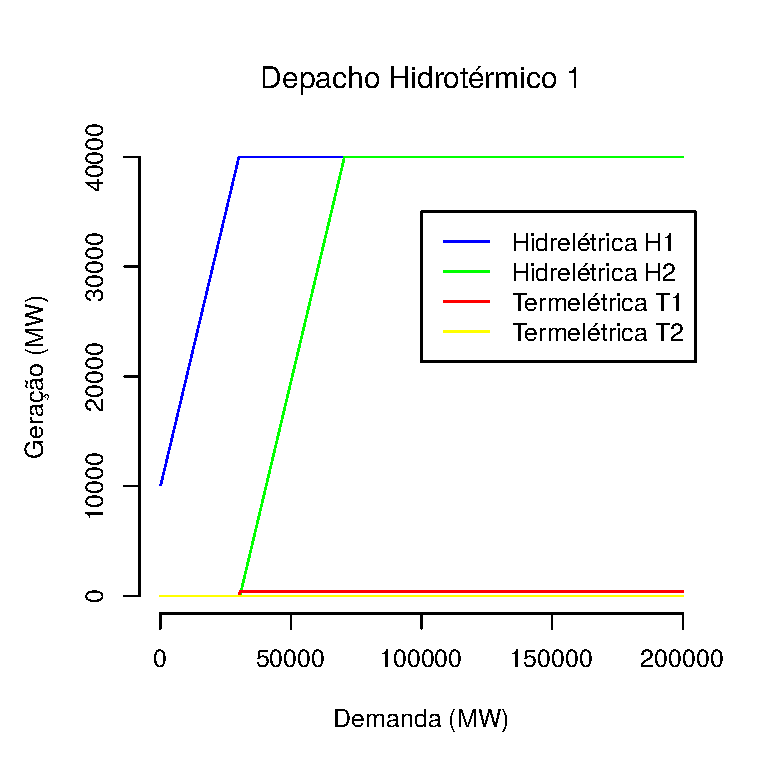
\includegraphics[width=5cm, height =5cm]{simulacaopb01pt10.eps}}
  \subfigure[Produtibilidade = 1,4]{
	\includegraphics[width=5cm, height =5cm]{simulacaopb01pt14.eps}}
\subfigure[Produtibilidade = 1,8]{
	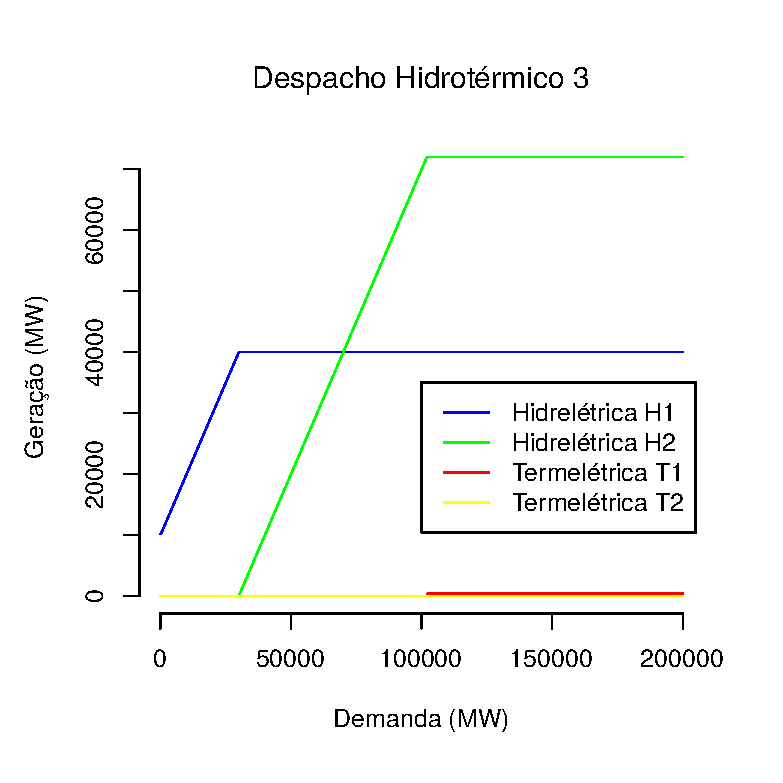
\includegraphics[width=5cm, height=5cm]{simulacaopb01pt18.eps}}
	\caption{Configura\c c\~ao de despacho para p = 0,1 e 1-p = 0,9}
\end{figure}
\section{CONCLUS\~OES}
O objetivo do presente estudo foi analisar o comportamento de um sistema hidrot\'ermico sobre varia\c c\~ao de demanda,
como metodologia utilizou-se a Programa\c c\~ao Din\^amica Dual Estoc\'astica (PDDE), o sistema foi
estruturado com duas hidrel\'etricas em cascata H1 e H2 e duas term\'eletricas associadas T1 e T2. Pelas simula\c c\~oes
verificou-se que as varia\c c\~oes na demanda podem alterar significativamente o comportamento de sistemas hidrot\'ermicos, mesmo com
os empecilhos da utiliza\c c\~ao de term\'eletricas notou-se que sua utiliza\c c\~ao ainda \'e fundamental para o
funcionamento do sistema, onde na simula\c c\~ao, T1 foi ativada antes que H2 para o primeiro caso, havendo
tamb\'em ativa\c c\~ao da termel\'etrica T1 para o segundo caso de estudo. Pela independ\^encia da term\'eletrica T1 no
sistema hidrot\'ermico uma vez que essa n\~ao \'e afetada pelo acoplamento temporal ou espacial, seu ponto de \'otimo
\'e atingido rapidamente, mesmo antes da hidrel\'etrica H2. O algoritmo de (PDDE) em nenhum momento da  simula\c c\~ao
solicitou a ativa\c c\~ao de T2, isso deve-se ao fato de T1 tem atingido seu ponto de \'otimo rapidamente,
impossibilitando as condi\c c\~oes de ativa\c c\~ao de T2. Nesse
 contexto, a (PDDE) foi uma metodologia com resultados favor\'aveis, uma vez que manteve a demanda do sistema com a
 ativa\c c\~ao de apenas uma termel\'etrica e no decorrer do processo a sua utiliza\c c\~ao permaneceu est\'avel,
 evitando-se que aumentos de demanda trouxessem preju\'izos de custo e ambiental. Contudo, o fato da necessidade da
 ativa\c c\~ao da term\'etrica T1 ocorrer antes da hidrel\'etrica H2, pode ser considerada tamb\'em uma desvatagem
 pelo aspecto do sistema da prioridade a sua ativa\c c\~ao. No geral o comportamento  do sistema foi esperado pela
 prioridade dada a utiliza\c c\~ao de H1, por outro lado pode-se observar como a independ\^encia das termel\'etricas
 afetaram o algoritmo da PDDE. O presente estudo est\'a longe de abordar todos os aspectos que envolvem a demanda em
 sistemas hidrot\'ermicos, existindo muitas caracter\'isticas a serem debatidas sobre o tema, por exemplo altera\c
 c\~ao de par\^ametros que permitam que o algoritmo de PDDE tenha uma prefer\^encia
 pelas hidrel\'etricas, \'e um dos aspectos relevantes. Por fim essa an\'alise justifica-se pela crescente preocupa\c c\~ao
 ambiental e pela necessidade de suprir a demanda por energia, sendo necess\'aria ao desenvolvimento da sociedade.

% ------------------------------------------------------------------------
\renewcommand{\refname}{REFER\^ENCIAS}

\begin{thebibliography}{99}
\fontsize{11}{0}\selectfont
\bibitem[Ag\^encia Nacional de Energia El\'etrica (ANELL)]{anell}
  AG\^ENCIA NACIONAL DE ENERGIA EL\'ETRICA (ANELL).
  {\em  Capacidade de Gera\c c\~ao do Brasil}.
  Dispon\'ivel em: \url {http://www2.aneel.gov.br/aplicacoes/capacidadebrasil/capacidadebrasil.cfm}.Acesso em : 19 de Julho.
  \begin{comment} 
\bibitem[]{benders}
  {\em Benders, J.F. Numer. Math. (1962) 4: 238.} 
  Dispon\'ivel em :\url {https://doi.org/10.1007/BF01386316.}
  Acessado em : 19 de Julho de 2019. 

\bibitem[Centro de Pesquisas de Energia El\'etrica (Cepel)]{cepel}
  CENTRO DE PESQUISAS DE ENERGIA EL\'ETRICA (Cepel).
  {\em DECOMP-MODELO DE PLANEJAMENTO DA OPERA\c c\~AO DE SISTEMAS HIDROT\'ERMCOS INTERLICADOS DE CURTO PRAZO}. Dispon\'ivel em:\url {http://www.cepel.br/pt_br/produtos/decomp-modelo-de-planejamento
  -da-operacao-de-sistemas-hidrotermicos-interligados-de-curto-prazo.htm}.
  Acessado em : 20 de Julho de 2019.
  
\bibitem[decomp]{decomp}
  MODELO DECOMP CEPEL.{\em Manual de Refer\^encia}.Dispon\'ivel em:
  \url {http://www2.aneel.gov.br/aplicacoes/noticias/arquivos/pdf/Manual_Referencia_DECOMP.pdf}.Acessado em : 20 de Julho de 2019.

\bibitem[The International Energy Agency (IEA)]{iea}
THE INTERNATIONAL ENERGY AGENCY (IEA).
{\em Global Engagement}.
Dispon\'ivel em:\url{https://www.iea.org/countries/Brazil/.}
 Acessado em : 20 de Julho de 2019.

 %\bibitem[termeletrica]{ter}
   %TOLMASQUIM, M. Energia Termel\'etrica: G\'as Natural, Biomassa, Carv\~ao, Nuclear, EPE: Rio de Janeiro, 2016.
  \end{comment}
\end{thebibliography}
\vspace*{-0.1cm}
% ------------------------------------------------------------------------

%For papers written in Portuguese or Spanish.

%\begin{center}
%  TITLE IN ENGLISH

%\end{center}

%\def\abstractname{Abstract}%

%\begin{abstract}
%   Abstract in english
%\end{abstract}

%\keywords{\em{Keywords in english}}

\end{document}
